\section{eo\-Fit\-Continue$<$ EOT $>$ Class Template Reference}
\label{classeo_fit_continue}\index{eoFitContinue@{eoFitContinue}}
Fitness continuation:.  


{\tt \#include $<$eo\-Fit\-Continue.h$>$}

Inheritance diagram for eo\-Fit\-Continue$<$ EOT $>$::\begin{figure}[H]
\begin{center}
\leavevmode
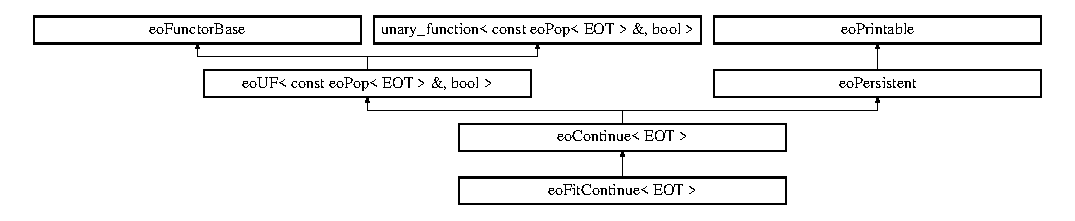
\includegraphics[height=2.52252cm]{classeo_fit_continue}
\end{center}
\end{figure}
\subsection*{Public Types}
\begin{CompactItemize}
\item 
typedef EOT::Fitness {\bf Fitness\-Type}\label{classeo_fit_continue_w0}

\begin{CompactList}\small\item\em Define Fitness. \item\end{CompactList}\end{CompactItemize}
\subsection*{Public Member Functions}
\begin{CompactItemize}
\item 
{\bf eo\-Fit\-Continue} (const {\bf Fitness\-Type} \_\-maximum)\label{classeo_fit_continue_a0}

\begin{CompactList}\small\item\em Ctor. \item\end{CompactList}\item 
virtual bool {\bf operator()} (const {\bf eo\-Pop}$<$ {\bf EOT} $>$ \&\_\-pop)
\begin{CompactList}\small\item\em Returns false when a fitness criterium is reached. \item\end{CompactList}\item 
virtual std::string {\bf class\-Name} (void) const \label{classeo_fit_continue_a2}

\end{CompactItemize}
\subsection*{Private Attributes}
\begin{CompactItemize}
\item 
{\bf Fitness\-Type} {\bf maximum}\label{classeo_fit_continue_r0}

\end{CompactItemize}


\subsection{Detailed Description}
\subsubsection*{template$<$class EOT$>$ class eo\-Fit\-Continue$<$ EOT $>$}

Fitness continuation:. 

Continues until the maximum fitness level is reached. 



Definition at line 36 of file eo\-Fit\-Continue.h.

\subsection{Member Function Documentation}
\index{eoFitContinue@{eo\-Fit\-Continue}!operator()@{operator()}}
\index{operator()@{operator()}!eoFitContinue@{eo\-Fit\-Continue}}
\subsubsection{\setlength{\rightskip}{0pt plus 5cm}template$<$class EOT$>$ virtual bool {\bf eo\-Fit\-Continue}$<$ {\bf EOT} $>$::operator() (const {\bf eo\-Pop}$<$ {\bf EOT} $>$ \& {\em \_\-pop})\hspace{0.3cm}{\tt  [inline, virtual]}}\label{classeo_fit_continue_a1}


Returns false when a fitness criterium is reached. 

Assumes pop is not sorted! 

Implements {\bf eo\-UF$<$ const eo\-Pop$<$ EOT $>$ \&, bool $>$} {\rm (p.\,\pageref{classeo_u_f_a1})}.

Definition at line 48 of file eo\-Fit\-Continue.h.

References eo\-Pop$<$ EOT $>$::nth\_\-element\_\-fitness().

The documentation for this class was generated from the following file:\begin{CompactItemize}
\item 
eo\-Fit\-Continue.h\end{CompactItemize}
